\documentclass[12pt]{article}

\usepackage[T1]{fontenc}
\usepackage[utf8]{inputenc}
\usepackage[russian]{babel}
\usepackage{xcolor}
\usepackage{minted}
\usepackage{graphicx}
\usepackage{float}
\usepackage[margin=1.5cm]{geometry}

\newminted{python}
{
frame=lines,
framesep=2mm,
baselinestretch=1.2,
bgcolor=darkgray,
fontsize=\footnotesize,
python3,
style=monokai,
rulecolor=white
}


\title{Разбор задач конкурса "Звёзды Кассиопеи"}
\date{20.05.2021}
\author{Надобных Дмитрий, Пугач Сергей, Чечеватов Роман}

\begin{document}
	\pagenumbering{gobble}
	\maketitle
	\pagenumbering{arabic}
	\newpage
	\section{Ручные задачи}
	Для решения данных задач не нужны никакие навыки программирования и они вам не сильно помогут. Вместо этого участникам предлагалось научиться искать информацию в файлах, анализировать их.
	\newpage
	\subsection{MP5}
	Эта задача засчитывалась как решенная после перехода по ссылке. Ничего сложного.

	\newpage
	\subsection{Автостоп}
	Как сказано в условии, ответом на данную задачу является ответ на Главный вопрос жизни, вселенной и всего такого. Вопрос этот был задан английским писателем Дугласом Адамсом в книге "The Hitchhiker’s Guide to the Galaxy", русским читателям известной как "Автостопом по галактике". 
	\linebreak
	Участники, читавшие этот роман могут спокойно ответить "42" и получить баллы, остальным придётся скопировать вопрос в Гугл и получить ответ в первом же результате.
	\linebreak
	Ответ: 42
	
	\newpage
	\subsection{Язык программирования}
	Для решения этой задачи участникам необходимо было изучить HTML-код страницы задачи. Для этого можно воспользоваться встроенными в браузер инструментами разработчика, или скачать страницу и открыть в текстовом редакторе. Независимо от выбранного способа, ответ находился в комментарии рядом с формой ввода ответа.
	\linebreak
	Ответ: flag\{html\_is\_the\_best\_language\}

	\newpage
	\subsection{Фотосессия}
	В данной задаче участникам давался для анализа JPG-файл с картинкой. Однако, такие файлы зачастую содержат в себе не только данные изображения, но и дополнительную информацию. Например, дату съемки, модель камеры, имя автора. И среди этой дополнительной информации и был спрятан флаг.
	\linebreak
	 Ответ: flag\{haha\_you\_thought\_it\_will\_be\_ccv\}

	\newpage
	\subsection{PI}
	Здесь участников просили ввести число Пи с некоторой точностью: строго заданное число знаков после запятой, не больше и не меньше. Достаточно точное число Пи можно взять на Википедии или, для пользователей Windows 10, Калькуляторе.
	\linebreak
	Отгадать необходимую точность можно с помощью метода проб и ошибок, или просто написав бота.
	\linebreak
	Ответ: 3.14159265358979323846264338327

	\newpage
	\subsection{Задача, которую невозможно решить}
	Вопреки сказанному в названии задачи, её возможно решить. Наличие решения этой задачи показывает, как внимательно участники прочитали инструкцию по работе с тестирующей системой. Ведь именно в разделе "Мануал", в подразделе "Обработка персональных данных", совершенно не к месту находилось предложение "Однако, для решения задачи, которую невозможно решить, вам нужно всего лишь отправить название конкурса". Остаётся лишь найти правильное с точностью до символа название. 
	\linebreak
	Ответ: Звёзды Кассиопеи
	
	\newpage
	\subsection{Двадцать пятый кадр}
	В данной задаче участникам предлагался для анализа файл с видео. И хотя в метаданных на этот раз флага не было, там можно было обнаружить частоту кадров видео: 120 кадров в секунду. Это значит, что на экранах с частотой обновления 60 Гц и менее (а таких на момент проведения конкурсов подавляющее большинство) немалая часть кадров просто не будет отображаться. Но зачем же авторы дали видео с таким большим числом кадров, зная, что часть из них не будет показана? Неужели они хотели что-то там спрятать? Да. Смотрим видео покадрово и на 817 кадре замечаем серый текст на сером фоне.
	\linebreak
	Ответ: flag\{you\_have\_great\_eyes\}

	\newpage
	\subsection{Eglishman}
	В очередной раз отправляемся в Гугл (Яндекс, Bing, DuckDuckGo, Рамблер, Поиск Маил.Ру, ...) чтобы узнать, как сервер может узнать местоположение/страну/язык пользователя и узнаём, два основных способа: по IP и по предпочитаемому языку пользователя. Методом проб и ошибок, испробовав все платные и бесплатные VPN-сервера узнаем, что в данной задаче IP ничего не значит. Остаётся вариант с языком. Браузер внутри запроса отправляет информацию о предпочитаемом языке веб-страниц. В настройках браузера выставляем предпочтение на английский, отправляем что угодно в качестве ответа и получаем баллы.

	\newpage
	\subsection{1C}
	В следующей задаче на анализ содержимого файла участникам был дан файл Excel. Изучив свойства файла или создав новый лист, можно обнаружить, что кроме видимого листа с многозначащим названием "Лист1" в книге есть ещё два: "Лист2" и "Лист3". В Microsoft Office Excel жмём ПКМ по списку листов, "Показать...", "Лист2". Изучаем содержимое ранее скрытого листа рядом с красивой картинкой аэродинамических характеристик коровы обнаруживаем флаг.
	\linebreak
	Ответ: flag\{cow\_aerodynamics\_power\}

	\newpage
	\subsection{Машина времени}
	Снова скачиваем приложенный файл. Распаковываем архив, наряду с привычными, но ничем не примечательными файлами обнаруживаем папку .git. Или не обнаруживаем, если у вас не включено отображение скрытых файлов. В таком случае, включаем, потому что без него заниматься поиском скрытой информации весьма непросто. В любом случае, закинув название папки в Гугл получаем понимание, что авторы дали вам Git-репозиторий. Git - одна из систем контроля версий, то есть позволяет отслеживать и сохранять изменения файлов, откатываться к предыдущей версии. Скачиваем Git, устанавливаем. Делаем коммит с помощью \verb|git commit -a| , видим, что после последнего сохранения состояния файлов. Откатываемся к предыдущему коммиту \verb|git checkout a23d2c7|, смотрим содержимое когда-то бывшего удаленным файла, находим флаг.
	\linebreak
	Ответ: flag\{wayback\_machine\_master\}

	\newpage
	\subsection{Плёночный фотоаппарат}

	\newpage
	\subsection{Плёночный фотоаппарат 2}

	
	\newpage
	\section{Задачи на использование ботов}
	Для начала рассмторим общую для всех ботов часть: работу с сетью. Мы использовали для написания ботов \verb|Python 3| и библиотеку \verb|requests|. Ничто не мешало вам использовать другие варианты, а незнание любого из них компенсируется длиной конкурса и доступностью всё того же Гугла.

	Импортируем библиотеку и задаём константы: 
	\begin{pythoncode}
# -*- coding: utf-8 -*-                           # Волшебное слово, чтобы использовать кириллицу
import requests                                   # Импортируем requests 

login = 'login'                                   # Сохраняем логин и токен
token = '23847634320439b65adafb7e3fefff802b1cde0a1b2977c3fe299a6dd111e4ce'
host = 'https://fetefot763.eu.pythonanywhere.com/'
	\end{pythoncode}
	
	Теперь нужно разобраться, как браузер отправляет запросы на сайт. Открываем панель разработчика и изучаем (см. рисунок \ref{fig:browser1}): 
\begin{figure}[H]
	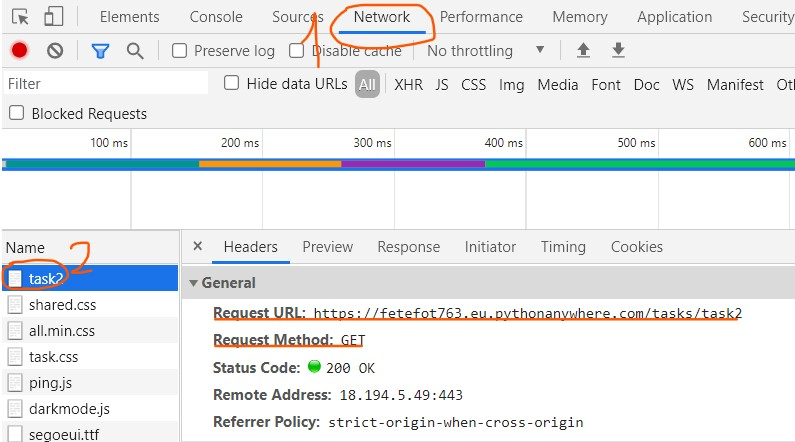
\includegraphics[width=\linewidth]{BrowserNetworkAnalysis0.jpg}
	\caption{Изучение процесса получения страницы браузером.}
 	\label{fig:browser1}
\end{figure}
	
	Видим, что браузер отправляет GET-запрос на страницу задачи. Продолжаем изучение, проматываем вниз (см. рисунок \ref{fig:browser2}):
	
\begin{figure}[H]
	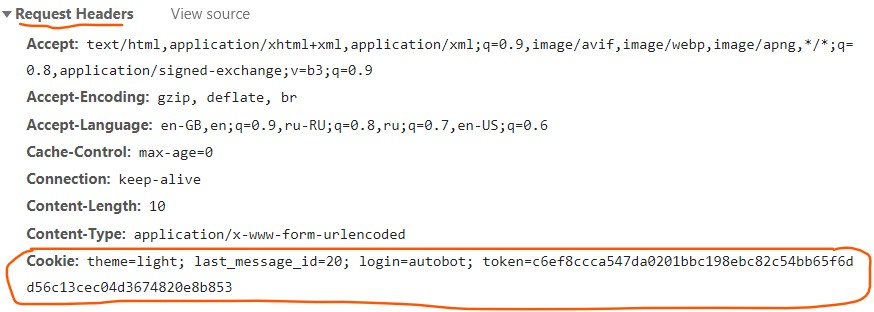
\includegraphics[width=\linewidth]{BrowserNetworkAnalysis2.jpg}
	\caption{Изучение отправляемых браузером cookie-файлов.}
 	\label{fig:browser2}
\end{figure}
	
	Теперь видим, что браузер отправляет cookie-файлы, чтобы получить страницу. Почитав в мануале обнаруживаем, что для работы необходимо только две печеньки: \verb|login| и \verb|token|. Их значения сохраняем к себе и используем дальше.
	\linebreak
	Используя полученные знания мы можем написать функцию получения задачи. Функция - это обособленный фрагмент кода, выполняющий узкую задачу.
	\linebreak
	Для задач, где в приложении дан текст, мы можем получить этот текст прямо со страницы задачи:

	\begin{pythoncode}
# Для текстовых задач (на примере задачи №1 - Водолей)
def get_data():                                   # Объявляем функцию
    text = requests.get(                          # Отправляем запрос
        host + 'tasks/task1',                     # На страницу задачи
        cookies={'login': login, "token": token}  # С cookies авторизации
    ).text                                        # И сохраняем текст ответа в переменную text
    return text                                   # Возвращаем text
	\end{pythoncode}

	Заметим, что функция \verb|get_data| возвращает нам весь HTML-код страницы. Нам же нужно только приложение к заданию. Приложения всегда находятся в блоке с \verb|id="task_data"|. И не содержат блоков внутри. Пользуясь этим, создадим новую функцию для извлечения этого приложения:

\begin{pythoncode}
def get_text_from_data(data):
    marker_beg = '<div id="task-data">'     
    marker_end = '</div>'
    ind_beg = data.rfind(marker_beg) + len(marker_beg)  # Индекс начала содержимого блока в строке
    ind_end = data[ind_beg:].find(marker_end)           # Индекс конца содержимого блока в строке
    text = data[ind_beg:ind_beg + ind_end]              # Сохраняем содержимое блока в переменную
    return text                                         # Возвращаем text
	\end{pythoncode}

	Следует чётко понимать, какую задачу вы решаете и какие функции из приложенных вам следует использовать. Так, функция получения текста задачи вернет мусор, если текста в задаче не окажется. А что произойдет с вашей программой при попадании внутрь мусора никому не известно.
	\linebreak
	\linebreak
	Если же в приложении дана ссылка на файл, то его нужно скачать. Тогда функция может ничего не возвращать: результат запроса уже сохранен в файл и будет прочитан из него.

\begin{pythoncode}
# Для файловых задач (на примере задачи №2 - WinRar 3000)
def get_data():                                   # Объявляем функцию
    requests.get(                                 # Отправляем запрос
        host + 'tasks/task2',                     # На страницу задачи
        cookies={'login': login, "token": token}  # С cookies авторизации
    )
    with open('2.zip', 'wb') as file:             # Создаём и открываем файл 2.zip для записи
        file.write(                               # Записываем в файл
            requests.get(                         # Отправляем запрос
                host + f'task-generated-content/2/task2_{team_id}.zip', # За файлом
                cookies={'login': login, "token": token} # С cookies авторизации
            ).content                             # Записываем в файл ответ на запрос
        )
	\end{pythoncode}

	Теперь проанализируем отправку браузером нашего решения задачи. Напишем что-нибудь в поле ответа и нажмем кнопку отправки. Посмотрим, что же нам показывает браузер в уже знакомой панели (см. рисунок \ref{fig:browser3}):
	
	\begin{figure}[H]
		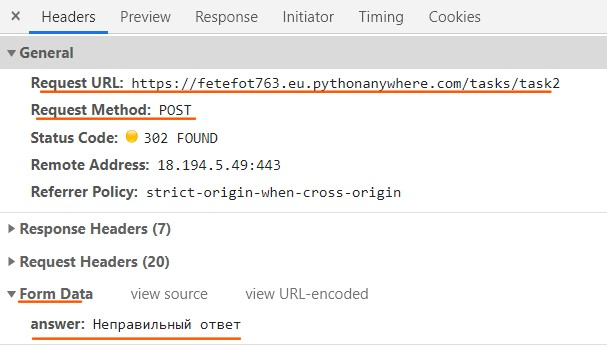
\includegraphics[width=\linewidth]{BrowserNetworkAnalysis3.jpg}
		\caption{Изучение отправки браузером ответа на задачу.}
	 	\label{fig:browser3}
	\end{figure}	
	
	Видим, что браузер отправляет запрос всё на ту же страницу, он уже POST. В запрос браузер включает \verb|данные формы|, содержащие поле \verb|answer| со значением, которое мы только что вписали в поле ввода ответа. Ещё замечаем что браузер снова отправляет cookie. Он их вообще всегда отправляет.
	\linebreak
	Напишем функцию отправки ответа в данных формы:

	\begin{pythoncode}
def send_data(data):                              # Объявляем функцию
    requests.post(                                # Отправляем запрос
        host + f'tasks/task{task_id}',            # На страницу задачи
        data={'answer': data},                    # С данными формы
        cookies={'login': login, "token": token}  # И cookies авторизации
    )
 	\end{pythoncode}
	
	На этом работа с сетью завершается. Остаётся только в правильном порядке вызывать наши функции:
	
	\begin{pythoncode}
# Для текстовых задач
if __name__ == '__main__':                        # Если запущен именно этот файл
    while True:                                   # Вечный цикл
        txt = get_text_from_data(get_data())      # Получаем текст задачи
        res = solve(txt)                          # Решаем задачу и сохраняем ответ
        send_data(res)                            # Отправляем ответ
 	\end{pythoncode}
	
	\begin{pythoncode}
# Для файловых задач
if __name__ == '__main__':                        # Если запущен именно этот файл
    while True:                                   # Вечный цикл
        get_data()                                # Получаем данные
        res = solve()                             # Решаем задачу и сохраняем ответ
        send_data(solve())                        # Отправляем ответ
 	\end{pythoncode}
 	
 	Просто вставить этот код себе и запустить у вас не получится: функция \verb|solve| неопределена. Реализацию этой функции мы рассмортим отдельно для каждой задачи.

	\newpage
	\subsection{Школьный конкурс компьютерной графики на тему "Программирование"}
	Здесь ничего решать не нужно, нужно просто отправить \verb|29 апреля|. Тогда фукция \verb|solve| может просто возвращать эту строку, без каких-либо вычислений.
	\begin{pythoncode}
def solve(txt):
    return '29 апреля'
 	\end{pythoncode}
 	
 	\newpage
	\subsection{Водолей}
	
	\newpage
	\subsection{WinRar 3000}
	
	\newpage
	\subsection{Никита Егоров}
	
	\newpage
	\subsection{Цветовод}
	
	\newpage
	\subsection{Кадровое агенство}
	
	\newpage
	\subsection{Вечеринка}
	
	\newpage
	\subsection{Календарь}
	
	\newpage
	\subsection{Я - Гуль}
	
	\newpage
	\subsection{Рукой подать}
	
	\newpage
	\subsection{Emoji Warrior}
	
	\newpage
	\subsection{CuSo4}
	
\end{document}